
\newrefsection

%\textbf{B1.a. Extended Synopsis of the scientific proposal}

\chapter{B1.a. Extended Synopsis of the scientific proposal}\label{part1}

\eu{(max 5 pages)}

\eu{The Extended Synopsis should give a concise presentation of the scientific
proposal, with particular attention to the ground-breaking nature of the
research project and the feasibility of the outlined scientific approach.
Describe the proposed work in the context of the state of the art of the field.
References to literature should also be included. References do not count
towards the page limits. It is important that this extended synopsis contains
all essential information including the feasibility of the scientific proposal
since the panel will only evaluate Part B1 at step 1.}

\section{Long-term vision and ground-breaking nature of the project}

\begin{framed}
\bf

\noindent\bf Social robots need a deep understanding of their social environment
to behave appropriately and adapt to their users' expectations; yet no
principled method exists to represent -- and therefore, reason -- on social
situations. This fundamentally hampers the progress of robots towards 
fully capable social agents.

The \project project aims at addressing that gap, both at the basic research
level, and at the real-world experimental level. The core idea enabling this
breakthrough, is to design and implement \emph{social embeddings}: compact, highly expressive
mathematical representations of arbitrarily complex social situations, built via
machine learning. Over the 5 years of the project, I will fully develop this
idea, characterizing how the semantics and dynamics of social situations are
represented, and how such embeddings enable a range of new social
capabilities that were considered until now out of reach.

\noindent Specifically, the \project project will investigate the following
two overarching research questions:

\begin{itemize}
        \item how to build compact, yet semantics-preserving, embeddings to
            represent arbitrary social and spatial environments for service
            robots.; how to fully characterize these embeddings, including their
            latent semantics;

        \item how to leverage these embeddings on real-world robots and
            applications to enable new complex socio-cognitive capabilities. In
            particular, I will research how social embeddings can support:

            \begin{itemize}
                \item context-appropriate behaviour learning and generation,
                    using attention-based and adversarial generative neural networks;
                \item contextualised lifelong adaptation of the robot's
                    behaviours, by augmenting existing interactive machine
                    learning techniques (`user in-the-loop' learning) with
                    representations of the social environment;
                \item automatic user engagement assessment;
                \item automatic detection of unexpected situations
                    based on discontinuities in the embedding space (for
                    instance, frustration, social norm violations, etc.)
            \end{itemize}

\end{itemize}

\noindent The long-term vision underpinned by these research questions is of
socially-useful robots which learn to become autonomous while continuously
adapting to the needs of their users. Social embeddings let robots build a
semantically accurate representation of their environment, enabling in turn
users to effectively teach context-appropriate behaviours to the robots. By
doing so, they actively shape the robots' roles and behaviours, based on
their actual, real-world needs and experience, while ensuring transparent
and ethical behaviours.

\vspace{0.4em}

\noindent Importantly, and because the development of socially-intelligent
robots has the potential of alienating their human users, \project also
includes a strong research component on Responsible Robotics. In particular,
the project will aim to contribute directly to the roadmap for Responsible
Robotics, specifically investigating the interplay between machine learning
applied to social robotics, transparency and human agency.

\end{framed}

%The service and companion robots that we are set to interact with in the coming
%years, are being designed and built today in labs and startups all over the
%world. How can we ensure 'by design' that they will have a net social utility?
%In other words: at the age of deep neural network and large language models,
%what are the conditions for ensure responsible social robots?
%
%\project will build the \textbf{new science required for robots to represent, reason and
%act in complex social environments}, with the goal of realising \textbf{a vision
%of social robots that enable humans and humans relationships to thrive}.
%\project is about creating the conceptual and technical frameworks required for
%safe and responsible social robots, intrinsically driven to foster stronger
%social interactions with and between humans.
%
%\textbf{\project main objective is, within 5
%years, to design, implement and demonstrate in the real-world the AI engine of a
%responsible socially intelligent robot}. Using the complex use-case of social
%isolation in elderly care centres, we will show that a social robot that
%implements Responsible Robotics principles, is accepted and adopted on the long
%term by the stakeholders, and can have a genuinely positive, long lasting,
%impact on the well being of older people.
%
%This objective is underpinned by two research hypotheses: (\textbf{H1}) for
%end-users to ascribe social utility and engage with the robot over long periods
%of time (months, years), the robot has to have its own long-term internal
%motivation to be socially helpful -- a \emph{social teleology}.
%
%(\textbf{H2}) Additionally, long-term acceptance also requires the
%genuine involvement of end-users in the shaping of the robot behaviours. As I
%have shown in my past research, this user engagement generate trust, feeling of
%ownership, and foster acceptance. Extrapolating from my laboratory result on
%interactive machine learning, I hypothesise that this process may lead to
%\emph{mutual accomodation} and eventually long term acceptance of a robot able
%to continuously adapt to the need of its users.
%
%To test and verify these two hypotheses in the real-world requires
%\textbf{breaking new ground in science and engineering}. Critically, we need to
%endow robots with a powerful way of representing and reasoning about their
%social environment.  \project aims at achieving this breakthrough by developing
%the mathematical models underpinning the recently discovered \emph{social
%embeddings}, and significantly expanding their expressiveness.
%

\subsection{Framing and scope}

AI and robots are emerging as key factors to successfully address modern societal
challenges, like the ageing society or increasing social isolation. In this
context, researchers in social robotics have the prime responsibility to ensure
that robots can understand and reason about their spatial and social environment
in such a way as to ensure a responsible and positive societal impact.

This can only be achieved if robots are endowed with the ability to represent
not only their physical environment, but also their social environment and
context. The \project project aims at designing, implementing and characterising
a radically novel method to achieve this goal, based on the concept of
\emph{embedding}: a low-dimensional, semantics-preserving, mathematical
representation of a high-dimensional input. Starting from a proof-of-concept of
\emph{social embeddings} that I recently published~\cite{lemaignan2024social},
\project introduces the concept of \emph{social embeddings}, that applies, for
the first time, the idea of building a compact numerical representation to the
complexity of social interactions and social dynamics.

\vspace{0.4em}

The scope of the project is ambitious: 


%\vspace{0.5em}
%\begin{itemize}
%
%    \item What are the conceptual, algorithmic and technical prerequisites to
%        design and implement such an autonomous \& responsible robots? in
%        particular, what social context understanding and (machine) learning
%        architectures are required to \textbf{enable long-term autonomy} and,
%        eventually, \textbf{engagement} between a robot and its end-users?
%
%    \item What are the conditions and methodologies enabling large scale data
%        acquisition of \textbf{real world, user-driven robots behaviours}? How
%        to then train robots to become \textbf{progressively autonomous}?  And
%        ultimately, how to balance \textbf{autonomy} of the robot with the
%        necessary \textbf{behaviour transparency} and \textbf{human oversight}?
%
%    \item What are the public expectations with respect to the role of social
%        robots, and how can we \textbf{collaboratively design}
%        \textbf{autonomous}, yet \textbf{responsible, beneficial, socially
%        acceptable robots}?
%
%\end{itemize}
%
%\vspace{0.5em}
%\noindent From these questions, I derive the following four objectives that are
%the guiding principles of my research program, both in the short term, and at a
%10-15 years horizon:

\subsection{Methodology}

Actual utility and long-term acceptance requires genuine involvement of the
end-users at every step of the design process. This is at odds with the common,
engineering-centered practise of first developing robots and algorithms \emph{ex-vivo}, in
lab, and then placing a (semi) final product in the hands of the users, hoping
for adoption. Adoption, however, is the result of a long process of \emph{mutual
modelling}~\autocite{sabanovic2010robots}, where
the social role of the robot is slowly constructed from its real world, in-context
usage.

This foundational insight requires the conceptual framing and development of new
research methodologies.  I have started to explore these questions in some of my
previous work~\autocite{senft2016sparc,winkle2019effective,winkle2021leador},
and my research program aims at significantly developing this line of research
to tackle more complex, long-term application domains.

One of the major challenge arising with more complex application domains is
however the combinatorial growth of the problem space. Indeed, none of the
current control paradigms or cognitive modelling techniques are able to
successfully predict context- and task-appropriate sequences of behaviours
for socially-useful autonomous robots.

\vspace{0.4em}

My research programme aims at tackling this challenge with two key insights: (1) the
representation complexity of the social and spatial environment of the robot 
can be dramatically reduced by treating it as an \emph{embedding} problem and
applying modern machine learning techniques (like GANs) to design and compute
\emph{social embeddings}; (2)
modern transformers and attention-based~\autocite{vaswani2017attention} machine learning
architectures have demonstrated long-term modelling
capabilities on complex language domains~\autocite{ouyang2022training} that could
in principle be equally applied to action sequence generation for
robots. Initial explorations of this second insight have started to
emerge~\autocite{brohan2022rt,vemprala2023chatgpt}, but none of these early research
efforts consider the complexity of human interactions.

\vspace{0.4em}

My research program will research how these insights can be effectively
operationalized, with a scientifically ambitious
and highly technical work program. It includes basic research and conceptual
framing; extensive, beyond-state-of-art, technical developments; and an
ambitious experimental program, centered on long-term `user in-the-loop' data
collection via field deployments of social
robots in public spaces -- and primarily in the healthcare and elderly care
environment.


\subsection{Work plan outlook}

My research program could begin rapidly, using publicly available resources,
including machine learning architectures like Transformers, combined with open-source
pre-trained Large Language Model backbones; and state-of-art HRI tools like
ROS4HRI~\autocite{mohamed2021ros4hri} to represent in real-time the social
environment of the robot. While long and complex data collection campaigns would
have to be organised, and training infrastructure would need to
be designed, I expect initial results in the first 3 to 5 years.

This is also a long-term vision: on the one hand, the rapid pace of progress
of technology (novel deep machine learning architectures, novel HRI tools for
human and scene understanding) continuously opens novel investigation
venues; one the other hand, the success of my research vision hinges on
real-world, long-term experimental work: deploying robots in the healthcare
sector, creating the conditions for adoption by the end-users, running
long-term deployments with the end-users are long terms aims
,... these research activities will take
place over long period of time.

\subsection{Importance and impact}

My research program has the potential to be groundbreaking: until now,
autonomous social robots have had little real world success. Experiments and
deployments have been mostly limited to constrained application domains, where
rigid action policies (scripts, task planners) could be sufficient. State-of-art
robots however fail to handle the complexity and unpredictability of real world
environments (like the ones encountered in the healthcare domain). In addition,
these systems see poor field adoption due to several factors including
difficulty of use, wrong expectations, perceived complexity.

This research program is also important: as socially assistive robots quickly
develop, it is critical to equip ourselves with a deeper understanding and
intellectual framing of what social robots \emph{could} and \emph{should} be,
paving the way for their much broader adoption in the coming years: I will
actively contribute to this aim, by leading the design and implementation of
socially-intelligent robots that are socially useful, acceptable in the
long-term, and ethically responsible, but also by furthering my engagement to
interdisciplinary work, and broad engagement with the society and policy makers.







%%%%%%%%%%%%%%%%%%%%%%%%%%%%%%%%%%%%%%%%%%%%%%%%%%%%%%%%%%%%%%%%%%%%%%%%%




%How this general
%principle translates into specific guidelines and algorithms -- while taking into
%account the principles of a responsible AI -- is the central
%contribution of Work Package 1.

% This socially-driven goal forms what we call a \emph{social
%teleology}. its own goals have this objective can only be achieved if the
%robot is \textbf{socially-driven}: the robot's behaviours must be driven by the
%intention to support positive human-human interactions. 


I frame these hypotheses with the idea of \textbf{robot-supported human-human
interactions}, a novel conceptual framework to `think' the future human-robot
interactions. I will co-construct this framework through large scale public
engagement: for a whole year, I will deploy the \project robot within the City
Lab of Bristol's science centre \emph{WeTheCurious}, relinquishing the control
of the robot to the visitors themselves. Tasked with remotely operating the
robot to assist fellow visitors, I will accompany them in `inventing by doing' a
new grammar of social interactions: what does it mean for a robot to help? How
to do so in the dynamic, messy, environment of a science centre? What are acceptable
behaviours? Can we see new social norms emerge? At the end of this experiment,
we expect 1000s of people to have had experienced -- and co-designed -- how
robots should interact with humans in a positive, helpful way, and each of these
experiences will contribute to uncovering and designing the basic principles of
social interaction for robots. This work is the focus of WP1.

While most of the interactions in the science centre will be short-lived, two further
large scale experiments will take place over the course of the project: a
one-year experiment in one of Bristol's Special Education Needs (SEN) school,
helping 250+ children with psycho-social impairments to develop their social
skills; a second one-year experiment at the Bristol's children hospital, where
the robot will join one of the wards where 30+ children with long-term conditions
stay for months, and engage with the children into playful social activities: telling
stories, triggering group activities with other children, providing additional
social presence. In both these experiments, the robot behaviours will be
co-designed with, and learnt from the end-users themselves: nurses, teachers,
parents, and where possible, the children themselves.


\begin{wrapfigure}[11]{l}{0.15\linewidth}
    \centering
    \vspace{-10pt}
    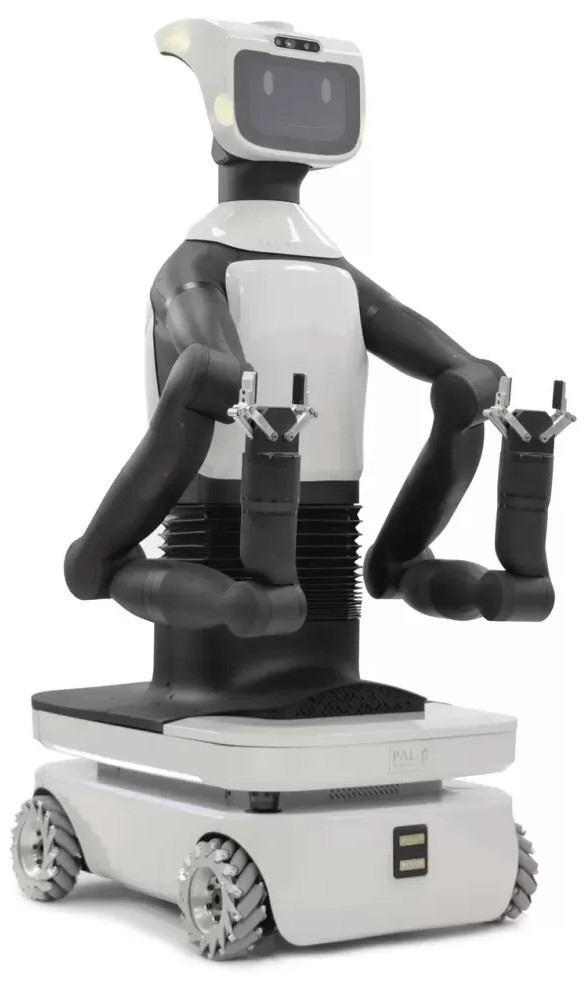
\includegraphics[width=\linewidth]{tiagopro}
    \label{fig|tiagopro}
\end{wrapfigure}

Importantly, \project focuses specifically on the \ul{AI engine} of the robot: I
will use an existing robotic platform (PAL Robotics TIAGo Pro, pictured on the left) and
develop and train the algorithms required to achieve autonomy and responsible,
long-term social utility. Indeed, after an initial training period, the robot
will be \emph{autonomous}: while the users will be provided tools to override
the robot decisions at any time (via both an app and touch sensors on the robot
itself), it will otherwise move and act on its own, without the need for
constant supervision. To this end, the robot will have ground-breaking
perception and modelling capabilities to represent the current social situation
(the focus of WP2), coupled with an innovative cognitive architecture designed
to combine internal social drives with domain-specific action policies learnt
from the end-users (WP4). The robot actions themselves are designed to be
limited to non-verbal communication mechanisms: non-verbal utterances using
sounds, gaze, joint attention, expressive motions. In WP3, my team will work
with a choreographer and a sound expert to create a new grammar of expressive
motions, combined with a novel modality based on \emph{soundscapes}: sound
landscapes that the robot can modulate to influence the mood of the social
environment (calm, excited, worried, etc.).

As a ground-breaking project, \project will assert and reinforce the European leadership in AI and
intelligent robotics, in line with the EU's strong societal values: by developing
socially responsible AI that guarantees, by design, long-term benefits to the
society. The very first task T1.1, spread over the first 4 years of the project,
specifically addresses and frames the ethical underpinnings of social robots,
and delivers the guidelines that we need to inform our future policies on social
robotics. Combined with beyond-state-of-the-art technological developments,
\textbf{the \project research programme will provide a major contribution in
securing a safe and responsible digital future in Europe}. 

Finally, \project is also about asserting and reinforcing the European
leadership in AI and intelligent robotics, in line with EU strong societal
values: a socially responsible AI, that guarantees, by design, long-term
benefits to the society. This requires leading major technological advances;
leading the development of the conceptual framework around socially intelligent
robots that we need to inform future policy making; but also \textbf{a strong
leadership to meaningfully involve the public at large in the design of these
technologies}. Through its objectives and methodology, \textbf{\project will
have a major contribution to building this capacity in Europe}. 


\section{Overview of the \project work programme}

Socially intelligent robots require unique, beyond state-of-the-art,
capabilities to \emph{(1)} understand the social interactions (social
situation awareness), \emph{(2)} autonomously decide the best course of action for
short-term and longer-term social influence, and \emph{(3)} perform the
appropriate social actions and exert said influence in an appropriate,
responsible manner.

Not only the required technology is itself beyond state-of-the-art (and will be
researched and integrated in WP2, WP3 and WP4), but the
interplay between technology, socio-cognitive psychology, privacy and ethics is
only starting to be researched and understood. \project offers an
strong vision and an ambitious, evidenced-based, methodology to significantly
advance our understanding of this multi-faceted problem.


\begin{itemize}
    \item \textbf{O1: conceptual framing} To construct a solid conceptual
        framing around the multidisciplinary question of responsible human-robot
        interactions, answering questions like: What should motivate the robot
        to step in and attempt to help? or: What social norms are applicable to
        the robot behaviours? Building on the extensive body of work on
        Responsible AI, I will investigate the basic principles of
        responsible robot-mediated social interactions, that must form the
        foundations of a socially useful robot, accepted and used in the long
        run.  Using user-centred design and participatory design methodologies,
        I will identify the determinants and parameters of a responsible social
        intervention, performed by a socially-driven robot, and formalise them
        in practical principles.

    \item \textbf{O2: physical-social representation and reasoning} To
        effectively and responsibly interact with its environment, the robot
        must first build a comprehensive and continuously updated model, from its
        spatial and physical configuration, to its social dynamics. I will
        design and develop a novel cognitive capability of artificial
        \emph{social situation assessment} to enable the robot to represent
        real-time social dynamics in its environment. I will achieve this
        breakthrough by combining existing model-based approaches \TODO{refs}
        (including my recent research on social state modeling \TODO{refs}, with
        the expressive power of the new \emph{social embeddings} that I have
        recently introduced.

    \item {\bf O3: goal-driven, responsible decision making} I aim to create
        robot behaviours that are perceived as purposeful and intentional
        (long-term goals), while being shaped by a user-created and
        user-controlled action policy.  I will integrate long-term social goals,
        arising from the interaction principles of \textbf{O1}, with the social
        modeling capability of \textbf{O2}, into a principled, goal-driven
        cognitive architecture, with responsible AI guarantees. The breakthrough
        will come from combining these long-term social goals with bottom-up
        action policies, designed and learnt from the end-users using
        human-in-the-loop attention-based machine learning.

        I want to specifically test the following two hypotheses: first, that
        long-term social goals, if suitably co-designed with the public and
        stakeholders and properly integrated into the robot as a \emph{social
        teleology}, will create the perception that the robot is intentional and
        purposeful. This will in turn elicit sustained engagement from its human
        users.

        Second, that human-in-the-loop machine learning can be used to ensure an
        additional layer of human oversight and a level of behavioural
        transparency.  Human-in-the-loop reinforcement learning -- as
        implemented in the SPARC approach that I have developed with my students
        and already used in complex social
        environments~\parencite{senft2017supervised,senft2019teaching,winkle2020insitu}
        -- relies on an end-user `teacher'. This teacher initially fully
        controls the robot (via teleoperation) while it learns the action
        policy, and then progressively relinquishes control up to a point where
        the robot is effectively autonomous. As I previsouly argued
        in~\textcite{senft2019teaching}, this approach leads to increased
        control and ownership of the system, and as a result, increased trust
        from the end-users.


    \item{\bf O4: ambitious field research} Finally, the last major objective of
        my research project is to demonstrate the effectiveness of my approach
        in complex, real-world conditions. This means deploying the socially
        interactive robots in existing social \emph{ecosystems} that are
        sufficiently complex and open to explore novel social interactions. My
        objective is also to show that this real-world deployment can be
        successfully driven by the `end-to-end' involvement of all the end-users
        and stakeholders: from defining the robot's role, from the different
        perspective of each end-user, to actually designing and `teaching' the
        robot what to do.


\end{itemize}


These objectives are investigated across five work-packages.

\subsection{WP1: \textbf{\wpOne}}

WP1 aims at establishing the conceptual and ethical framework around the idea of
\emph{robot-supported human-human interactions}. It does so by co-creating
patterns of interaction and norms with the general public, using a unique
combination of ethnographic observations and `crowd-sourced' interaction
patterns.

\begin{framed}
    \textbf{Main outcomes:} A theoretical framework to `think' the role of
    social robots and guidelines to inform policy making (including ethical
    implications); a set of operational \& co-created interaction principles; a
    large dataset of social human-robot interactions

    \textbf{Timeframe:} \textbf{Y1-Y3}; one senior post-doc (PD1)
with background in sociology of technology.
\end{framed}


\textbf{T1.1 -- Conceptual framing and ethics of robot-supported social
interactions}


The first task in WP1 is to research and define the conceptual framework around
questions like: what role should social robots have? Where
to set the boundaries of artificial social interactions? What does
`ethical-by-design', `responsible-by-design' mean in the context of social
human-robot interactions? 

Each of the field experiments (T1.2, T5.1. T5.2) will both \emph{build on} and
\emph{feed into} the framework developed in this task. In addition, four
two-days workshops with the \project Ethics Advisory Board, spread over the
duration of the project, will act as ethical milestones.

\textbf{T1.2 -- Crowd-sourced patterns of robot-supported social
interactions} The conceptual framework identified in T1.1 is translated
into a set of \emph{interaction design principles} and \emph{determinants} that
will together form a set of requirements and objectives for the socio-cognitive
capabilities and architecture developed in WP2 and WP4.

In order to anchor T1.2 into the reality and complexity of human social
interactions, and to involve the society at large into the design of these
patterns and norms, I will embed one \project robot in the Bristol Science
Centre WeTheCurious for a whole year (Y2). With the help of a researcher, the
visitors will be guided into tele-operating the robot to assist other visitors,
and, by doing so, co-design what a good robot helper should be. This will
generate the quantitative and qualitative data to inform questions like `what
role for the robot?', `when to intervene?', `what are the effective and
acceptable social influence techniques?'. It will also be a unique example of
crowd-sourcing at a large scale, with the general public, the interaction design
of social robots.  The generated dataset will also be used as data source in WP2
and WP3.

\textbf{Specific resources} The Bristol's Science Centre is fully committed to the
project, will include \project in its official programme of activities, and will
provide in-kind training for the \project researcher based at the centre.

%%%%%%%%%%%%%%%%%%%%%%%%%%%%%%%%%%%%%%%%%%%%%%%%%%%%%%%%%%%%%%%%%%%%%%%%%%%%%%%
% WeTheCurious
% 
% - one robot completelty controlled by children, one by adults
% 
% what to learn?
% 
% - when to approach? when to prompt? [example of the salesman/museum facilitator]
% - when is the right time to help/intervene or not? 'child being told off by
% parents -> not the right time!'
% - group interactions -> when to intervene? what about peer-pressure? eg what if
% I tell off one child in front of another?
% - break the barrier for participation. Japanese Journal paper -> facilitating students questions
% - impact on moral norms? what behaviours is acceptable?
% - what role for the robot? another mediator? a peer?
% - what can we do with that 'alien creature'
% 
% - robot taking one child to talk to the museum mediators ("I, robot, am  shy!
% would you come with me?")
% 
% - learning how to adjust behaviour based on personality
% - 'why do I behave like that with that person, and like this with that other
% person?'
% 
% - reinforcement learning instead of human-in-the-loop -> what reinforcement
% signal? engagement
% 
% - the robot that 'take sides': take side against the adults? -> bending in its
% role?
% 
% 
% - social embarassment
% - space for pretence: the robot can adopt an 'artificial role' as long as it is
% possible (accpetable/...) to pretend the robot is



\subsection{WP2: \textbf{\wpTwo}}


In WP2, the project addresses the key scientific and technical pre-requisites to
effectively deliver WP4's cognitive architecture; namely the perception and modeling of
the spatio-temporal and social environment of the robot. This includes spatial
characteristics (proxemics; group dynamics; complex, dynamic attentional
mechanisms); psycho-social determinants (social roles and hierarchies; social
groups; mental modelling; anthropomorphic ascriptions); temporal characteristics
(effects of novelty; dynamics of anthropomorphism and mental ascriptions; group
dynamics). I have investigated many of these socio-cognitive capabilities in
isolation (Table~\ref{pi-expertise}), and this WP is about
\emph{integrating} them into a coherent perceptual subsystem, significantly
extending the state-of-the-art~\cite{lemaignan2017artificial, baxter2016cognitive}.

\begin{framed}
    \textbf{Main outcomes:} A complete pipeline for spatio-temporal and social
    situation assessment, build as open-source ROS nodes, and able to map in
    real time the physical and social environment of the robot.

    \textbf{Timeframe:} \textbf{Y1-Y4}; one post-doc (PD2) in social
signal processing/machine learning/cognitive modelling.
\end{framed}

\textbf{T2.1 -- Hybrid situation assessment and knowledge representation} This
task builds the foundational spatio-temporal and symbolic perception and
representation system for the robot. It will integrate the state-of-the-art in
spatio-temporal situation assessment that I have previously
developed~\cite{lemaignan2018underworlds, sallami2019simulation} with recent
advances in data-driven semantic labelling (for instance, using 4D convolution
nets like MinkowskiNet~\cite{choy20194d}), and a symbolic knowledge base (like
my own ontology-based one~\cite{lemaignan2010oro}) in order to create a coherent
system of representations for the cognitive architecture of the robot.

\textbf{T2.2 -- Multi-modal human model} This task focuses on the processing and
modelling of social signals, extending existing techniques, both model-based
(eg~\cite{gunes2017automatic,lemaignan2016realtime}) and data-driven based
(eg~\cite{bartlett2019what}). This task goes beyond the state-of-the-art by
looking specifically at resolving highly dynamical signals (like gaze saccades
and micro facial expressions). Required datasets will be drawn from my previous
work~\cite{lemaignan2018pinsoro}, as well as from the project experiments (T1.2,
T5.1, T5.2).

\textbf{T2.3 -- Interaction and group dynamics} Building on T2.2, T2.3
investigates the automatic understanding and modelling of group-level social
interactions~\cite{tapus2019perceiving}, including
$f$-formations~\cite{marshall2011using}, sociograms (as done
in~\cite{garcia2016hybrid} for instance), and inter-personal
affordances~\cite{pandey2013affordance}. This task builds on literature on 
social dynamics analysis (eg~\cite{durantin2017social,jermann2009physical,
martinez2019collocated}) to apply it to real-time social assessment by a robot,
itself embedded into the interaction.

\textbf{T2.4 -- Integrated model of the social environment} The integration of
the social cues from T2.2 and T2.3 results in a socio-cognitive model of the
social environment of the robot, that effectively extends the representation
capabilities of T2.1 to the social sphere. The result of T2.4 is an AI module
that implements a full social assessment pipeline, from social signal perception
to higher-level socio-cognitive constructs. T2.4 also includes a
focused experimental programme (based on the protocols designed by Frith and
Happé~\cite{frith1994autism}, that I introduce in~\cite{lemaignan2015mutual}) to
demonstrate in isolation the resulting socio-cognitive capabilities.


\subsection{WP3: \textbf{\wpThree}} 

Mirroring WP2's focus on understanding the social interactions, WP3 addresses the
question of social behaviour \emph{production}: how to create natural,
non-repetitive behaviours, engaging over a sustained period of time. The robot
behaviours will be exclusively non-verbal (non-verbal utterances, gaze, joint
attention, facial expressions and expressive motions), and will include
soundscapes as a novel non-verbal interaction modality.

\begin{framed}

    \textbf{Main outcomes:} A new method to automatically design complex and
    non-repetitive social behaviours, with a focus on non-verbal communication;
    research on soundscapes as a novel non-verbal modality for human-robot
    interaction.

    \textbf{Timeframe:} \textbf{Y2-Y5}; one post-doc (PD3) in machine learning/learning from
demonstration.

\end{framed}

\textbf{T3.1 -- Behavioural baseline} T3.1 establishes a baseline for behaviour
generation, by surveying and implementing the current state of the art
(behaviours library, activity switching~\cite{coninx2016towards}). This
baseline will enable early in-situ experimental deployments, while also
providing a comparison point for T3.2.

\textbf{T3.2 -- Generative neural network for social behaviour production}
\project aims at significantly advancing the state of the art in this regard, by
combining two recent techniques: (1) generative neural networks for affective
robot motion generation~\cite{marmpena2019generating,suguitan2020moveae} (with
training data created with an expert choreographer); (2) interactive machine
learning in high-dimensional input/output spaces, where I have shown with my
students promising results for generating complex social
behaviours~\cite{senft2019teaching, winkle2020couch} that fully involve the
end-users~\cite{winkle2018social}. Modulating (1) with the learnt features of
(2), I target a breakthrough in robots' social behaviours generation: the
generation of non-repetitive, socially congruent and transparent social
behaviours (including gestures but also gazing behaviours and facial
expressions).

\textbf{T3.3 -- Non-verbal behaviours and robot soundscape} In task T3.3, we
introduce a novel non-verbal interaction modality for robots, based on
soundscapes: soundscapes are about creating a sound environment that reflects a
particular situation; they also have been shown to be an effective intervention
technique in the context special needs
interventions~\cite{greher2010soundscape}. The soundscapes that I will create
are `owned' by the robot, that can manipulate ithem itself, eg to create an
approachable, non-threatening, non-judgmental, social interaction context, or to
the establish the interaction into a trusted physical and emotional safe-space
for the user.

\textbf{Specific resource}: these soundscapes will be co-designed with Dr.
Dave Meckin, an expert on sound design for vulnerable children, who also works
at the host institution.

\subsection{WP4: \textbf{\wpFour}}

In WP4, I will design a novel socio-cognitive architecture for the social
robots, and implement it on the IIT R1 robot.  WP4 will integrate together the
modeling capabilities and behaviour production developed in WP2 and WP3, with a
dual action policy: a policy driven by a social teleology (eg an artificial
intrinsic motivation to act socially), and a policy learned through
human-in-the-loop machine learning. This WP is high-risk/high-gain: while sustaining
long-term engagement in a principled way remains one of major scientific
challenge in social robotics~\cite{hoffman2019anki}, the WP suggests a very novel
approach to goal-driven socio-cognitive architectures, with the potential of
unlocking long-term social engagement by endowing the robot with its own
intentionality~\cite{wiese2017robots}, while maintaining human oversight.

\begin{oframed}
    \textbf{Main outcomes:} An integrated cognitive architecture for social
    robots, driven by both long-term social goals, and machine-learnt action
    policies; a reference open-source implementation, enabling long-term
    autonomy on the IIT R1 robot.

    \textbf{Timeframe:} \textbf{Y1-Y5}; one post-doc (PD4) in cognitive
    robotics; one PhD student (PHD1).

\end{oframed}

\textbf{T4.1 -- A social teleology for robots} The idea of a \emph{teleological}
(ie goal-driven) robot architecture for social interaction is very novel
(existing literature on teleological robots only focuses on simple cognitive
systems~\cite{oudeyer2005playground,forestier2017unified}). This task designs
and implements such an architecture on the R1 robot. It first identifies from
the interaction patterns and determinants uncovered in T1.2 \emph{interaction
principles}, that are then mapped into \emph{long-term interaction goals}, capable of
driving the robot actions over a period of time.

\textbf{T4.2 -- Learning from humans to achieve `by-design' responsible \&
trustworthy AI} Building on my recent results on human-in-the-loop social
learning~\cite{senft2017supervised,senft2019teaching,winkle2020couch}, this task
implements the mechanics to allow human end-users to progressively teach the
robot a domain-specific social policy.  This task also qualitatively researches
how human-in-the-loop machine learning enables a more trustworthy AI system, by
involving the end-users in the creation of the robot behaviours, resulting in
explainable behaviours for the end-users.

\textbf{T4.3 -- Integrating a socially-driven architecture for long-term
interaction} Building on my previous work on cognitive
architecture~\cite{lemaignan2017artificial}, this task brings together, in a
principled manner, the perceptual (WP2) and behavioural
(WP3) capabilities of the robot, as well as the social policies created in T4.1 and
T4.2. T4.3 will specifically look at long term autonomy, including long-term
social goals, cognitive redundancy, and behavioural complexity.

T4.3 will also develop the arbitration mechanism that combines the robot's
social teleology (T4.1) with the human-taught action policy (T4.2). This
arbitration mechanism will build on research on reinforcement learning for
experience transfer~\cite{madden2004transfer} that enables the re-assessment of
a policy (here, our intrinsic motivation) based on previous experience (here,
the human-taught policy).

\subsection{WP5: \textbf{\wpFive}}

Finally, WP5 aims at convincingly demonstrating the importance and positive
impact that socially-driven, socially-responsible robotics may have. The
experimental work of \project will be organised around two ambitious long-term
studies, in complex, real-world environments: a network of special educative
needs (SEN) schools, and the Bristol Children's Hospital.

These environments also put the project in the unique position of actually
delivering high societal impact: I anticipate 30+ hospitalised children, and 250
SEN-educated children to directly benefit from the project, exploring how robots
can have a net social utility, while being accepted as effetive tools by field
practitioners. Both these deployments will take place within the strict ethical
framework established in T1.1.

\begin{oframed}

    \textbf{Main outcomes:} Two long-term deployments of a social robot in
    real-world, high impact environments demonstrating long-term acceptance and
    social utility; large (anonymous) datasets of complex, real-world
    human-robot interactions.

    \textbf{Timeframe:} \textbf{Y3-Y5}; one post-doc (PD4, shared with WP4).

\end{oframed}

\textbf{T5.1 -- A robot companion to support physical, mental and social
well-being in SEN schools} This task aims at demonstrating robot-supported
social interventions within Bristol's network of SEN schools.  During a one-year
period (Y3), the robot will be based in schools, with interventions co-designed
with the teachers, the parents and the students, both through preliminary
focus groups and in-situ machine learning.

The envisioned interventions include: initiating group games; enquiring students
about their well-being; co-teaching material with teachers; fostering
interaction situations between the children.

\textbf{Specific resources:} The task will be supported by local SEN researcher
Dr. Nigel Newbutt, who has a long track record and on-going research
partnerships with Bristol's special needs schools.


\textbf{T5.2 -- A robot companion to support isolated children during their
hospital stay} Over the course of this second, one-year long (Y4)
experiment, my team will deploy one \project robot in the long-term condition
paediatric ward at the Bristol Children's Hospital.  Using a \emph{mutual shaping}
approach~\cite{winkle2018social} to design the role of the robot with the
different stakeholders (nurses, doctors, parents, children), I will
experimentally investigate how a social robot can support hospitalised children
with long-term conditions. The robot's role will revolve around facilitating
social interactions between possibly socially isolated children, by fostering
playful interaction amongst children, within the ward.

\textbf{Specific resources:} Several preparatory meetings already took place
with the head of the hospital education service J. Bowyer, who will support the
project, granting access to the long-term conditions ward, and sponsoring the
project through the hospital-specific ethics process.


\section{Capacity of the Principal Investigator to deliver on the work programme}

While the project is ambitious, I am in a unique position to deliver on the
\project work plan. I already have established international recognition in
human-robot interaction and have likewise demonstrated strong leadership by
leading research teams in three different institutions (see Sections B1.b and
B1.c below). Importantly, as illustrated in Table~\ref{pi-expertise}, the
breadth of my interdisciplinary research covers the scientific expertise
required by the project, providing me with a unique overall perspective and
understanding of the domain. I am also a technology expert, with major software
and hardware contributions to the robotic community (see Section B1.c). As such,
I have a excellent grasp of the technical feasibility of the proposed work.


\begin{table}[h]
    \centering
    \caption{\small PI's domains of expertise relevant to the \project project}
    \begin{tabular}{rp{0.6\linewidth}}
        \toprule
        %\bf Expertise domain                  & \bf Corresponding publications by PI          \\
        %\midrule
        \textbf{Psycho-social underpinnings of HRI} \\  
        human factors & \small anthropomorphism~\cite{lemaignan2014dynamics}, cognitive
        correlates~\cite{lemaignan2014cognitive}, social influence~\cite{winkle2019effective} \\
        trust, engagement, social presence & \small \cite{flook2019impact,lemaignan2015youre,fink2014which,irfan2018social} \\
        theory of mind & \small perspective taking~\cite{ros2010which, warnier2012when}, social mutual modelling~\cite{lemaignan2015mutual,dillenbourg2016symmetry} \\
        \midrule
        \textbf{Social signal processing}\\
        non-verbal behaviours & \small attention~\cite{lemaignan2016realtime},
        child-child dataset~\cite{lemaignan2018pinsoro}, internal state decoding~\cite{bartlett2019what} \\
        verbal interactions & \small speech recognition~\cite{kennedy2017child}, dialogue grounding~\cite{lemaignan2011grounding} \\
        \midrule
        \textbf{Behaviour generation} \\
        social behaviours & \small \cite{lallee2011towards}, verbal interactions~\cite{wallbridge2019generating, wallbridge2019towards}, physical interactions~\cite{gharbi2013natural} \\
        interactive reinforcement learning & \small \cite{senft2017leveraging,senft2017supervised, senft2019teaching} \\
        \midrule
        \textbf{Socio-cognitive architectures} \\
        architecture design & \small \cite{lemaignan2017artificial, baxter2016cognitive,lemaignan2014challenges,lallee2012towards, mallet2010genom3} \\
        knowledge representation & \small
        ontologies~\cite{lemaignan2010oro, lemaignan2013explicit} \\    
        spatio-temporal modelling & \small object
        detection~\cite{wallbridge2017qualitative}, physics-aware situation
        assessment~\cite{lemaignan2018underworlds,sallami2019simulation} \\
        \midrule
        \textbf{Fieldwork in HRI} & \small in
        classrooms~\cite{hood2015when, lemaignan2016learning, jacq2016building,
        baxter2015wider,kennedy2016cautious,senft2018robots}, at home~\cite{mondada2015ranger}\\
        %\midrule
        %Robot hardware design for interaction & \small \cite{ozgur2017cellulo, hostettler2016realtime} \\
        \bottomrule
    \end{tabular}
    \label{pi-expertise}
\end{table}

The project is ambitious, with an experimental programme that goes significantly
beyond the state of the art. It will provide a lasting scientific and
technical legacy, that extends well beyond the end of the fellowship. As a
high-risk/high-gain project, \project will also be a powerful enabler: by the
end of the fellowship, I will have established myself as a world-leader in the
emerging field of socially-driven, responsible autonomous robots, significantly
reinforcing the European capacity in this critical field for our digital future.



\newpage

\printbibliography



